\section{Methodology}

\begin{CJK*}{UTF8}{min}
\subsection{Corpus}
The corpus used in model experiment is called ``ene-corbocha-mainiti''.
It consists with 8,228 news articles, 53,224 unique words, and 2,226,147 tokens.
The sentence is also annotated with word segmentation, POS, and chunk dependencies that annotated by the tool called: CaboCha.
Therefore, the corpus is about 7.38 times larger than CoNLL-2003 English corpus which consists of 1,393 articles with 301,418 tokens.
Despite the larger corpus, there also has wide variety of name entities in total of 190 types.
However, as the corpus of Japanese language is arranged and distinguished in a hierarchy following ``Sekine's extended named entity hierarchy - 7.1.0 -''.
Worrying that the label could be very sparse result that model rarely learn something, we decided to group all sub-categories into one top-most of its class accordingly to represent the name entity of each name entity word.
Thus, result to the amount of label types to decrease to 26 tags: \textbf{God, Percent, Location, Latitude Longtitude, Product, Ordinal Number, Name Other, Numex Other, Multiplication, School Age, Timex, Age, Natural Object, Disease, Person, Organization, Facility, Color, Money, Point, Rank, Countx, Frequency, Measurement, Event, and Period}.
Furthermore, the model contains a lot of handcraft features such as Part-Of-Speech and Word-pronunciation.
Also, arrange in XML format and group by sentence, chunk, and token level respectively. Data format The corpus is collected and pre-processing into XML format annotated by \textless sentence \textgreater, \textless chunk\textgreater, and \textless tok\textgreater tag as shown in code listing \ref{lst:xmlcorpus}.

\begin{lstlisting}[language={XML}, caption={Corpus XML format}, label={lst:xmlcorpus}]
<sentence>
  <chunk>
     <tok id="0" feature="..." ne="O" ene="B-Game">WORD1</tok>
     <tok id="0" feature="..." ne="O" ene="I-Game">WORD2</tok>
     <tok id="0" feature="..." ne="O" ene="O">WORD3</tok> 
  </chunk>
  <chunk>
    <tok id="0" feature="..." ne="O" ene="O">WORD4</tok>
    <tok id="0" feature="..." ne="O" ene="O">WORD5</tok>
  </chunk> 
</sentence>
\end{lstlisting}
The attributes of each token consist of \textbf{id}, \textbf{features}, \textbf{ne}, and \textbf{ene} where each attribute represent by the following:
\begin{itemize}
    \item \textbf{id:} Token ID 
    \item \textbf{feature:} POS, base form, pronounce
    \item \textbf{ne:} Named entity tag with BIO format
    \item \textbf{ene:} Fine grained named entity tag with BIO format
\end{itemize}
However, ``ne'' is an automatically identified named entity by CaboCha while ``ene'' is a manually annotated name entity.
Therefore, ``ene'' is the gold named entity tag.
Furthermore, for each chunk of the sentence, we can extract another feature given one chunk is affected by its following Japanese particle word.
The Japanese particle word could be categorized into 8 groups:


\begin{enumerate}
    \item \textbf{Case markers 「格助詞」 (Kaku-joshi) -}
    Represents a semantic relation in a sentence.
    Thus, it would provided an information about relationship between each name entity in a sentence.
    Case markers are included 「が、の、を、に、へ、と、で、から、より」.
    \item \textbf{Parallel markers 「並立助詞」 (Heiritsu-joshi) -}
    Align two things together.
    This Japanese particle would improve the ability to detect multiple name entities in a sentence.
    This markers included 「か、の、や、に、と、や ら、なり、だの」.

    \item \textbf{Sentence ending particles 「終助詞」 (Shū-joshi) -}
     Adds meaning such as doubt, prohibition and impression about the end of sentences and phrases.
     This particle consist with 「か、の、や、な、わ、とも、かしら」.
     However, this particle not really helpful on name entity detection but could be used in a task such as sentiment analysis.

    \item \textbf{Interjectory particles 「間投助詞」 (Kantō-joshi) -}
     This particle consist with 「さ、よ、ね」 and is used for give an expression.
     Same as Sentence ending particles, this particle is not really helpful on name entity detection but could be one emphasizing features used in other task.
     
    \item \textbf{Adverbial particles 「副助詞」 (Fuku-joshii) -}
    Adverb as a whole for phrases, adverbs particles, etc.
    This particles consists of 「ばかり、まで、だけ、 ほど、くらい、など、なり、やら」.


    \item \textbf{Binding particles 「係助詞」 (Kakari-joshi) -}
    This particles is used to emphasize the meaning of attached word.
    It consists of 「は、も、こそ、で も、しか、さえ、だに」.
    Likewise, this particle given the information of subject and object in the sentence as well as provide an information of the attached word whether the previous attached word is either topic, add, or exclusive expression in the context.

    
    \item \textbf{Conjunctive particles 「接続助詞」 (Setsuzoku-joshi) -}
    Express the semantic relation between sentence and sentence.
    Same as Sentence ending particles and Interjectory particles, this particle type is not really helpful on name entity detection but could be used in other task such as finding a relationship from sequence-to-sequence.
    This particles consists of 「ば、 や、が、て、のに、ので、から、ところが、けれども」.
    
    \item \textbf{Phrasal particles 「準体助詞」 (Juntai-joshi) -}
    Convert various words to a phrase as a whole.
    This particle usually used for grouping a same typical words together.
    Thus, it emphasizes the possibility of word using this particles to be the same name entity type or related.
    This particles consists of 「の、から」.

\end{enumerate}

\begin{figure}[!h]
\centering
  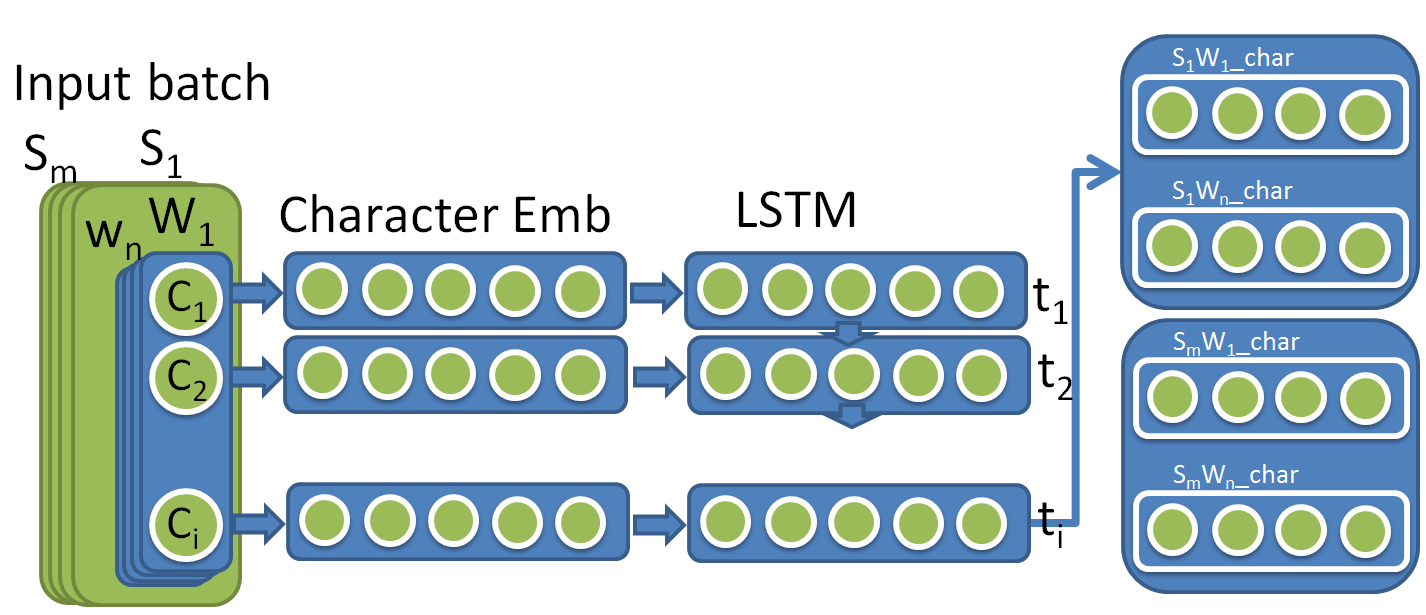
\includegraphics[scale=0.3]{character_encoder.png}
  \caption{Character-Encoder level.}
  \label{fig:chaenc}
\end{figure}

\subsection{Model}
\subsubsection{Character-Encoder level}
Input in this level are character indexes of each word from sentences.
As illustrates in Figure \ref{fig:chaenc}, \textbf{S} stands for a sentence from \textbf{1} to \textbf{m} for one input batch.
\textbf{M} stands for a word from \textbf{1} to \textbf{n} for one sentence.
Finally, \textbf{C} stands for a character from \textbf{1} to \textbf{i} for one word.
This input connected with a Character-Embedding level which will provide vector for each character.
As the main goal is to create a small and fast learning model as much as possible, the BiLSTM could be redundant to Word-Encoder level extracted features as switching of a character ordering would automatically count as a new word.
Thus, the output of Character-Embedding layer is connected to uni-direction LSTM which will accumulated and provided a vector for each word according to each sentence via it final hidden state output as \textbf{S\textsubscript{1-m}W\textsubscript{1-n}} char.
In addition, the experiment also applied on the filtering input character.
The filtering input character is the idea we proposed to improve accuracy, or at least accelerate a learning process.
Given that a name entity usually be \textbf{Noun} and the task is to seek only name entities within sentences, any word which is not \textbf{Noun} could be neglect.
The Character-Encoder level could be useful in such a case where there is a set of characters that could be used to identify a name entity for an organization same as ``CO.'', ``LTD.''in English.
As for Japanese, 「本」 character sometime could represent a location such as 「日本」(Japan) or a person/organization such as 「宮本、山本」(Muramoto, Yamamoto).


\begin{figure}[!h]
\centering
  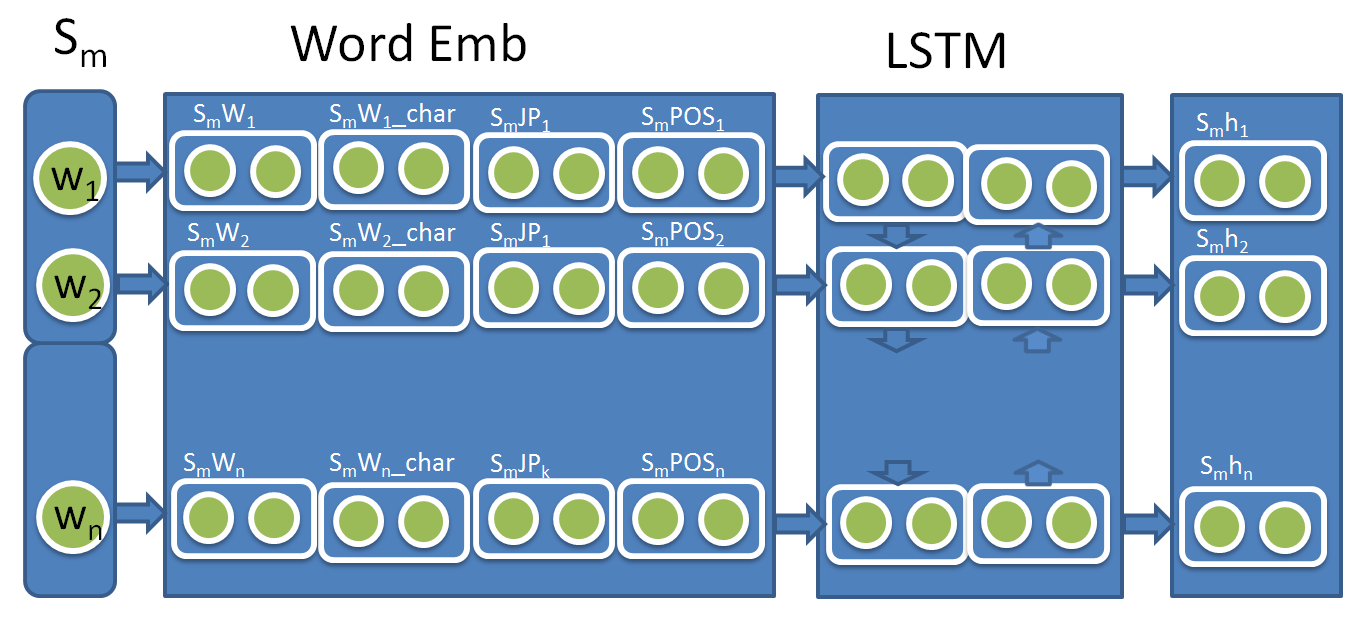
\includegraphics[scale=0.3]{word_encoder.png}
  \caption{Word-Encoder level.}
  \label{fig:winenc}
\end{figure}


\subsubsection{Word Encoder level}
This level is applied with various combination features inputs such as Japanese particle types (JP) as mentioned in the previous section, and Part-of-speech (POS).
As illustrate in Figure \ref{fig:winenc}, there are several chunk in one sentence.
Initially, consider input sentence of sentence \textbf{m} is \textbf{S\textsubscript{m}}, each word is an input that connected to its embedding layer to generate its vector from word \textbf{1} to \textbf{n} as \textbf{S\textsubscript{m}W\textsubscript{1-n}}.
Furthermore, each Part-of-speech is corresponded to each word and connected with its own embedding layer which result in \textbf{S\textsubscript{m}POS\textsubscript{1-n}}.
Finally, each Japanese particle types is considered by the last word of each chunk from \textbf{1} to \textbf{k}.
The chosen Japanese particle type then past its own embedding layer result in a vector \textbf{S\textsubscript{m}JP\textsubscript{1-k}}.
These features are concatenated with the previous level vector \textbf{S\textsubscript{m}W\textsubscript{1-n}}\_char to provide a new input which will feed to BiLSTM to figure the relationship between each word from both directions.
The output from Bi-directional LSTM for each word is collected as a vector \textbf{S\textsubscript{m}h\textsubscript{1-n}}.



\begin{figure}[!h]
\centering
  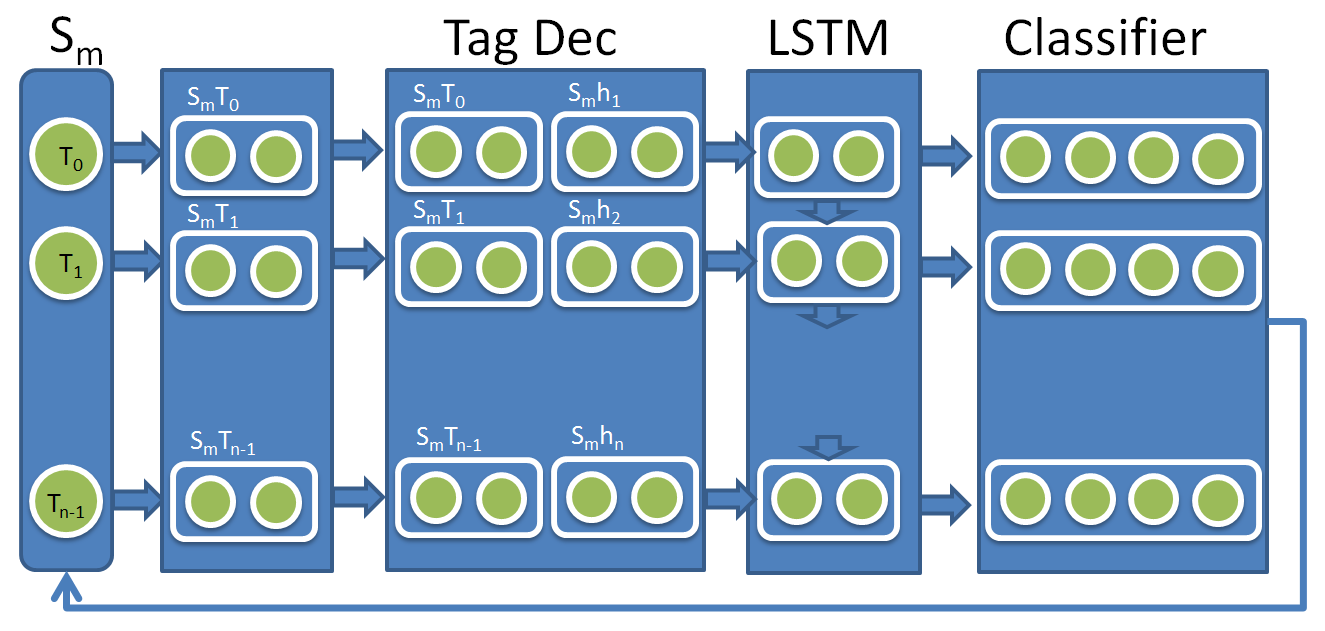
\includegraphics[scale=0.3]{tag_decoder.png}
  \caption{Tag-Decoder level.} 

  \label{fig:tagdec}
\end{figure}

\subsubsection{Tag-Decoder level}
Tag Decoder level is the last part in the model.
Its input is a concatenate vector between the output vector of each word from the previous Word-Encoder level and the output from a tag embedding layer.
However, the input of tag embedding layer is quite crafty as it is a previous timestep of its tag index.
Therefore, to predict the second word's name entity of a sentence, the first word's name entity is used as a feature and so on.
The concatenation of this input then pass through LSTM layer and one last linear layer to finally determine the each word's label.
Hence, it means that the output of word \textbf{n} of sentence \textbf{m} is determined by tag \textbf{n-1} of sentence \textbf{m} \textbf{S\textsubscript{m}T\textsubscript{n-1}} and hidden vector n of sentence \textbf{m} (\textbf{S\textsubscript{m}h\textsubscript{n}}).

\subsection{Weighted categorical cross-entropy}
Unlike usual name entity detection task on other work, ene-corbocha-mainiti corpus contains 26 name entity tags.
As a result, the model suffers greatly from an imbalance tags problem.
Also, a sampling method to adjust each label equally is likely impossible, as NLP task usually treat each input data as a sequence.
Thus, chosen Weighted categorical cross-entropy as a loss function
seem to be a correct logical decision.
An equation used for calculation such weight is described in following: 

\begin{equation} \label{eq1}
W_l = \frac{
    \sqrt{
    \sum_{i=0}^{n} X_i^2
    }
}{X_l} 
\end{equation}

Although, the weighted Cross-Entropy is not something new.
The calculation of a proper weight never been defined even from a tutorial of Cross-Entropy (Boer, 2005) \cite{750fabedbacb467c8fafd98b87f77436}.
Provided a simplest yet effective way for weighted calculation to reduce the time consumption for training one model is also our goal to deliver a compact model.
Equation \ref{eq1} variable consists of \textbf{W\textsubscript{l}} as a weight of target label and \textbf{X} as an amount of each label in a training data, \textbf{n} is the number of classes and \textbf{X\textsubscript{l}} is an amount of that class label.
Thus, the equation is an inverse function of Euclidean norm.
Upon the task, the model should give high priority to the name entity detection.
As name entity tags are much lower than non-name entity tags in number, this function is one of the most well-known and befit to abruptly adjust the model when the erroneous prediction occurs in minor groups.


\begin{equation} \label{eq2}
\mathit{loss(S,tag)} = W_l[\mathit{tag}](- \mathit{S[tag}] + log(\sum_{\mathit{j}} \mathit{exp(S[j])}
\end{equation}

After achieve weight of each tag, the loss is calculated by Equation \ref{eq2}. 
Hence, \textbf{W\textsubscript{l}[tag]} is a weight of each tag, \textbf{S[tag]} represents a score on the correct tag, and \textbf{S[j]} represents each score achieved from class \textbf{0} to class \textbf{j} where \textbf{j} is a total class exists.
After summation of loss, the overall loss is divided by the number of prediction times to find an average. We believed that by this learning method. Once the model able to distinguish between minority group which obviously a name entity accurately, the other tag should not be hard to adjust later on. Therefore, the model could avoid such a local minima that could occurred when adjust itself to O-Tags.
\end{CJK*}